% !TeX root = ../../thesis.tex



With the method described in the algorithm \ref{alg:simil_1}, we created a figure where the metrics are presented with increasingly different datasets: Figure \ref{fig:lineplot}.
%Then we compared the difference in the metric across iterations, rendering figure \ref{fig:boxplot}.

\begin{landscape}

%TC:ignore
\begin{figure}[htbp]
\centering
\caption{Plot showing the decrease of the metric over increasingly changed datasets. The X axis represents the number of columns mutated. The Y axis represents the value of the metric and the hue represents the algorithm used to calculate the metric.}\label{fig:lineplot} 
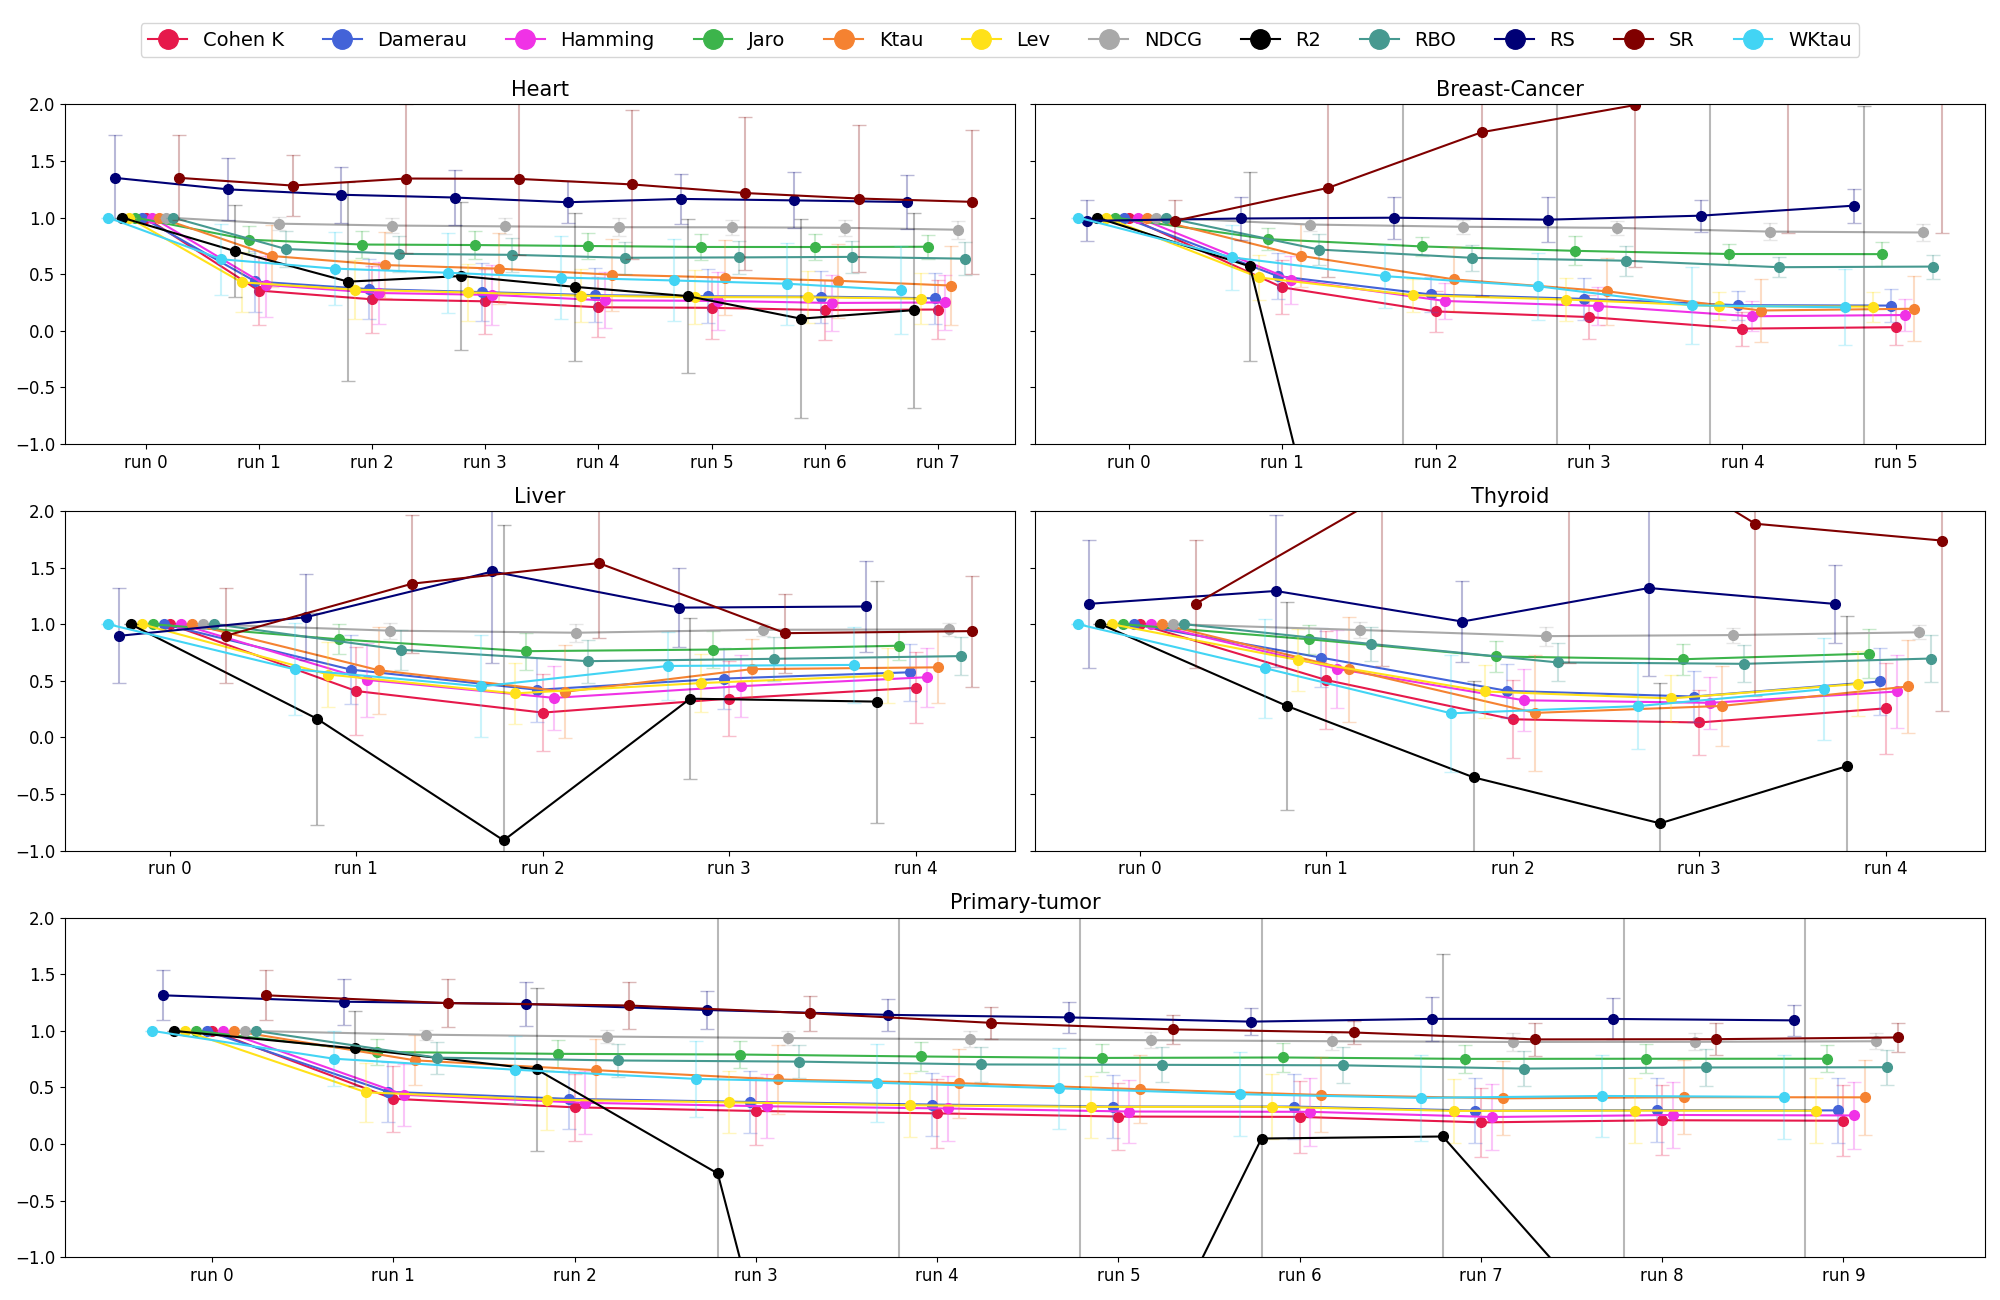
\includegraphics[scale=0.40]{figures/multiple_datasets_2.png}
\end{figure}
%TC:endignore
\end{landscape}

We also checked to see if the number of repetitions and how that impacts the variance of the scores. We found out that variance was low across most metrics, being the ones with higher variance was \ac{cc} and $R^2$ with values around 0.1 and Wktau and Ktau with values around 0.04 and 0.08. The others were less than 0.02. The data can be seen in figure~\ref{fig:nrruns}. As for the test for the synthetic and real dataset, the results are displayed in figure~\ref{fig:synth_result}. Values available in figure~\ref{fig:synth_heat}. This is the metrics distribution for the comparison of the 5 mentioned datasets and the synthetic counterpart generated as stated in the methods section.





%TC:ignore
\begin{figure}[htbp]
    \centering
    \caption{Heatmap showing the variance of different repetitions for every metric and the number of different columns changed. X is the metric. Y is the number of repetitions and the number of columns. This was obtained by getting the variance of all values from all datasets.  }\label{fig:nrruns} 
    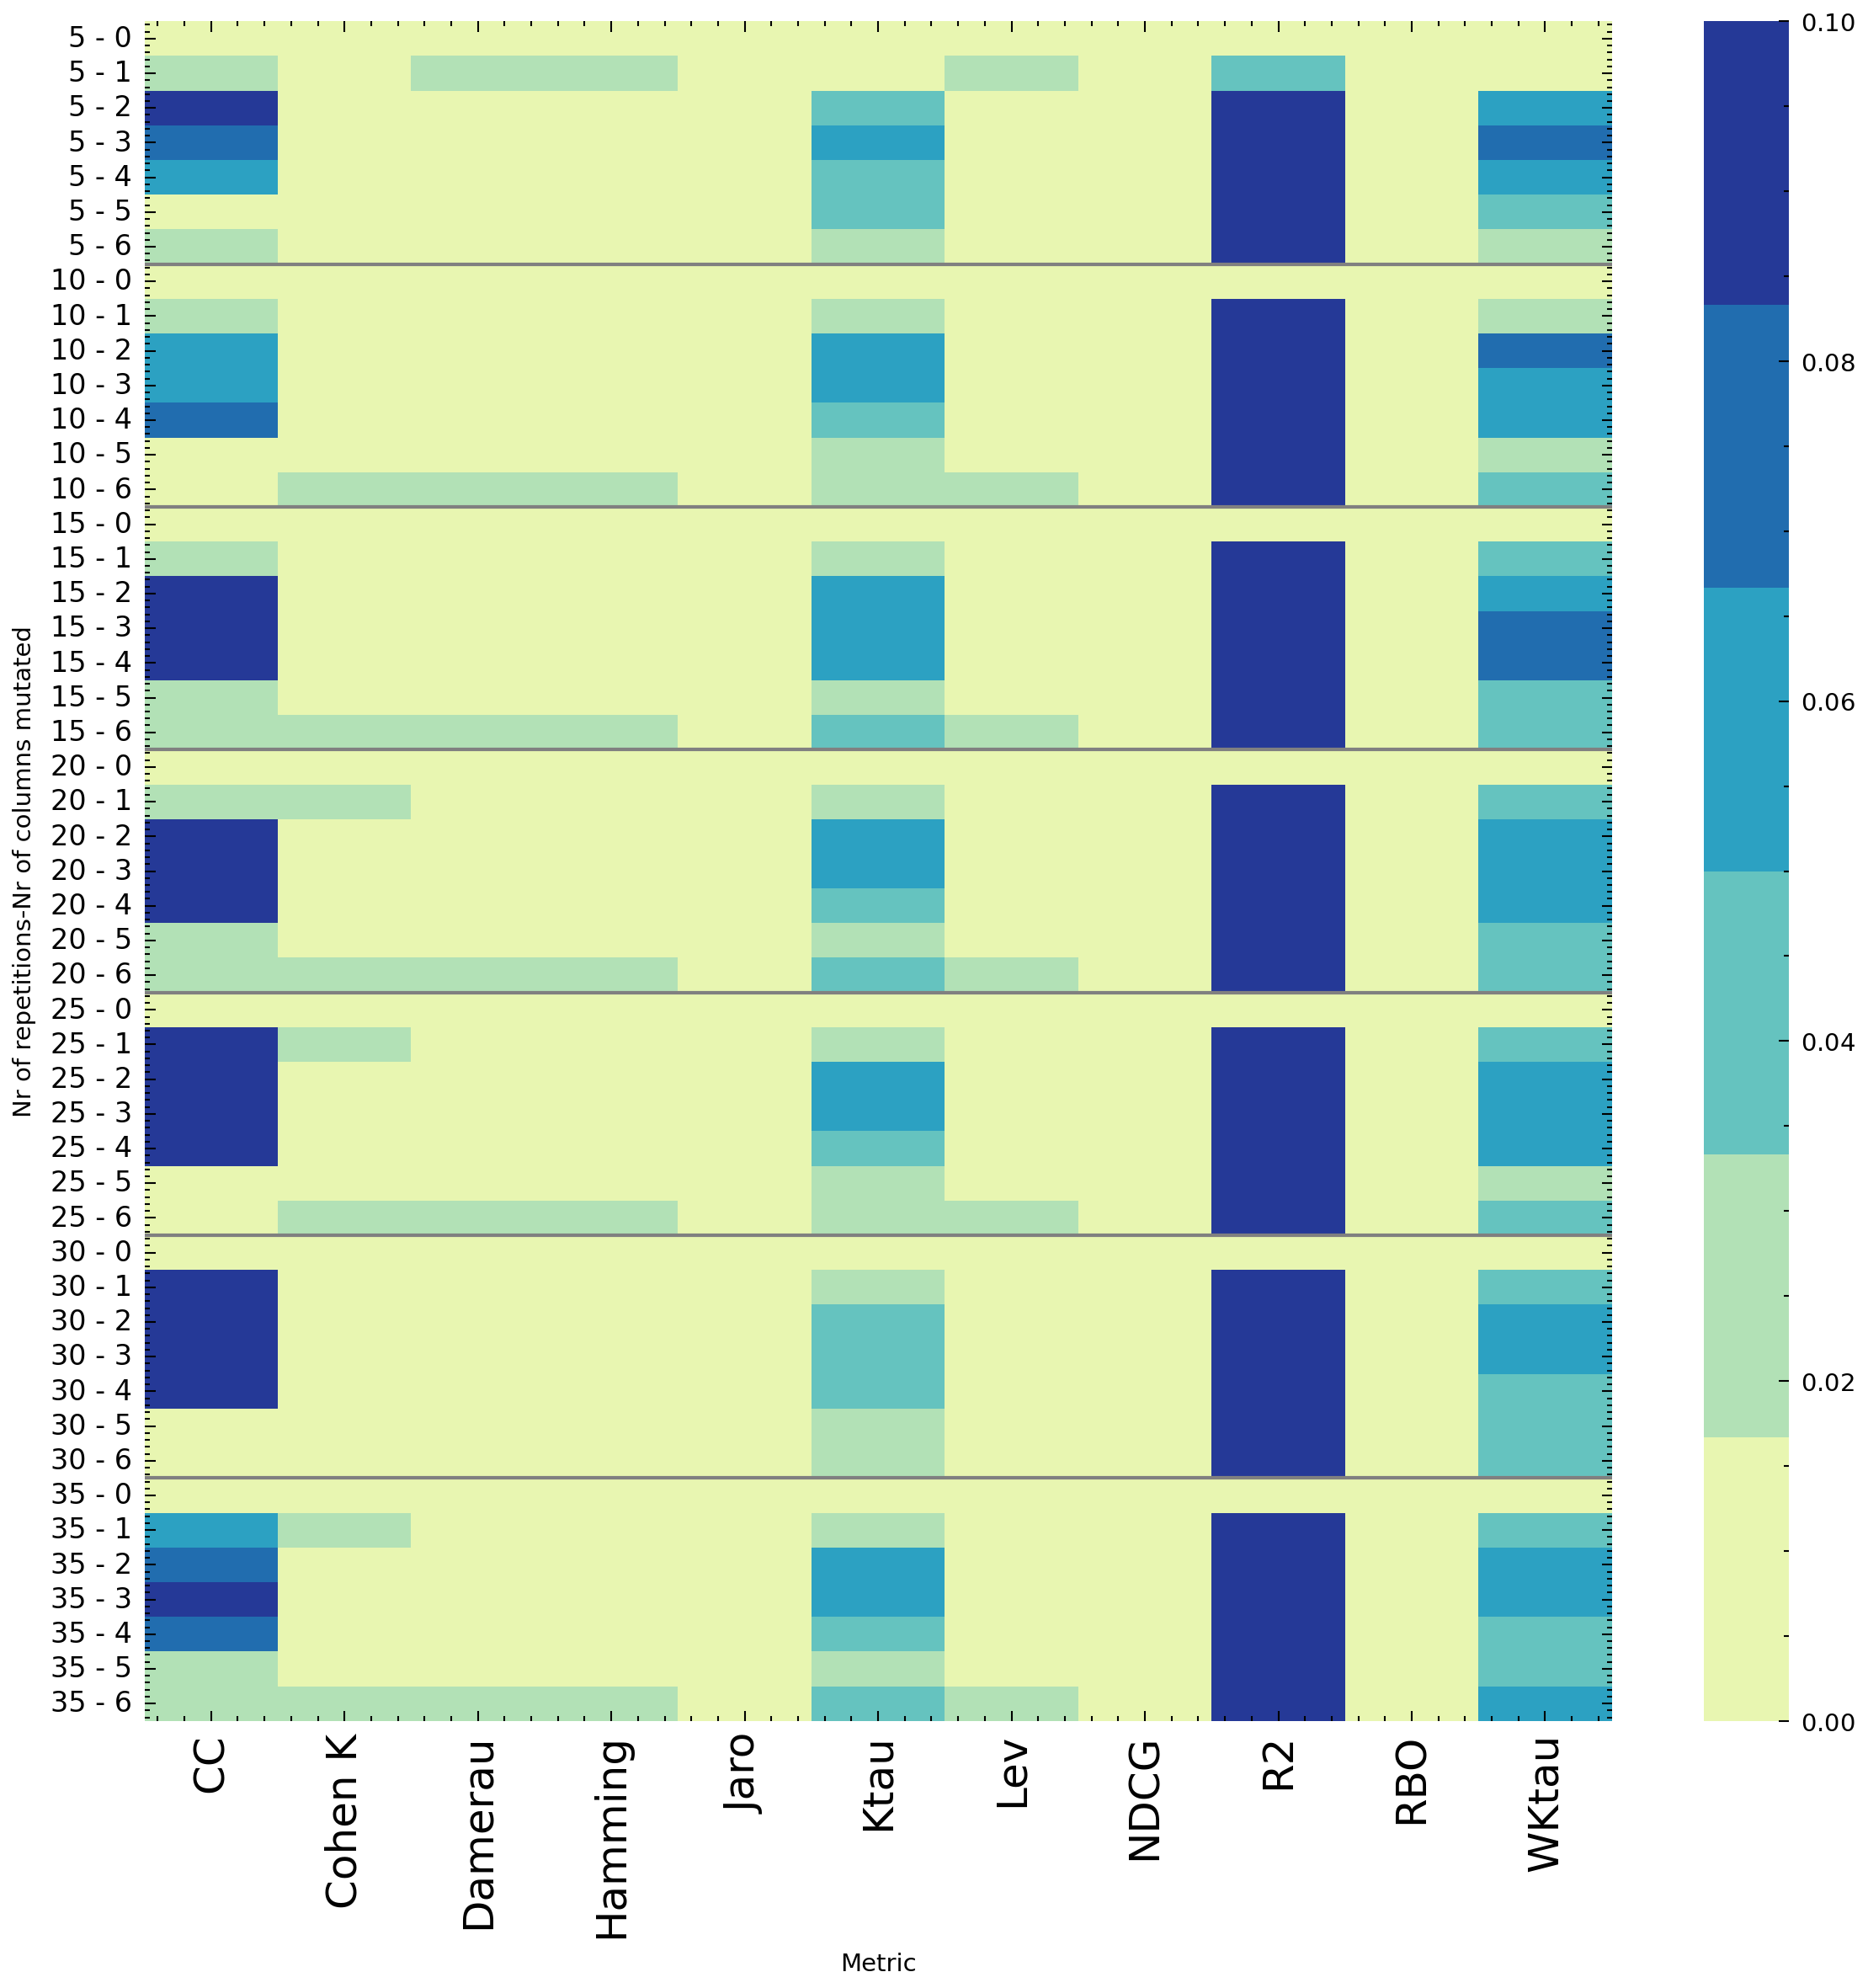
\includegraphics[scale=0.60]{figures/heatmap-runs.png}
    \end{figure}
    %TC:endignore


    \begin{figure}[htbp]
        \centering
        \caption{Values and comparison of the metrics results comparing 5 synthetic and real datasets across 3 different generation methods}\label{fig:synth_heat} 
       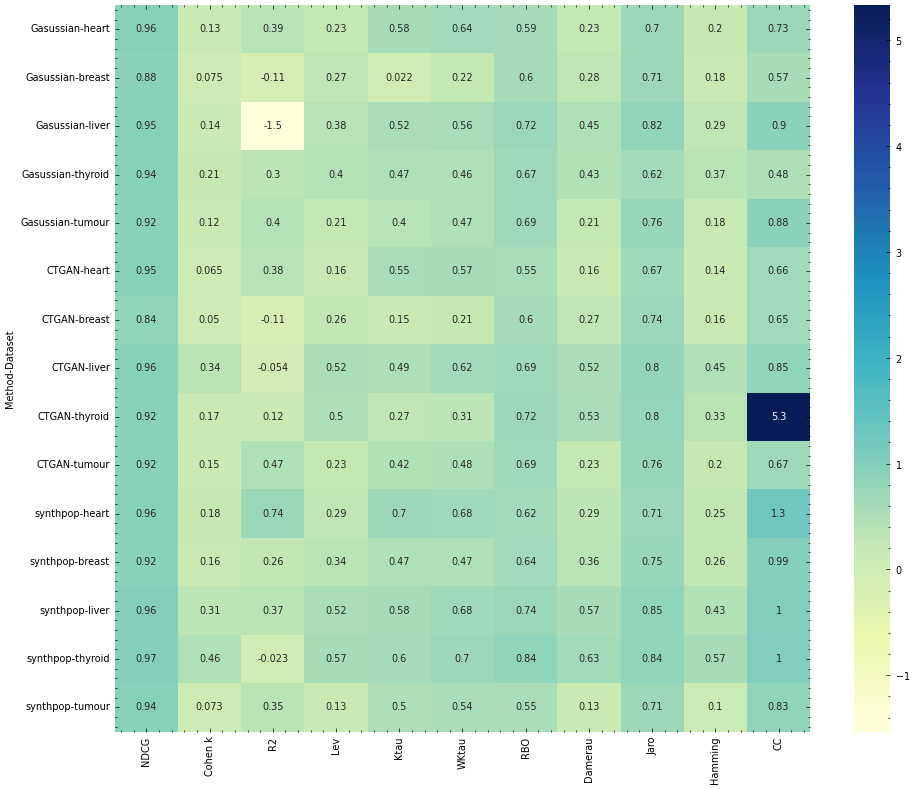
\includegraphics[scale=0.60]{figures/heatmap-synth.png}
        \end{figure}
    %TC:endignore

    
%TC:ignore
\begin{figure}[htbp]
\centering
\caption{Distributions of the metrics results comparing 5 synthetic and real datasets across 3 different generation methods}\label{fig:synth_result} 
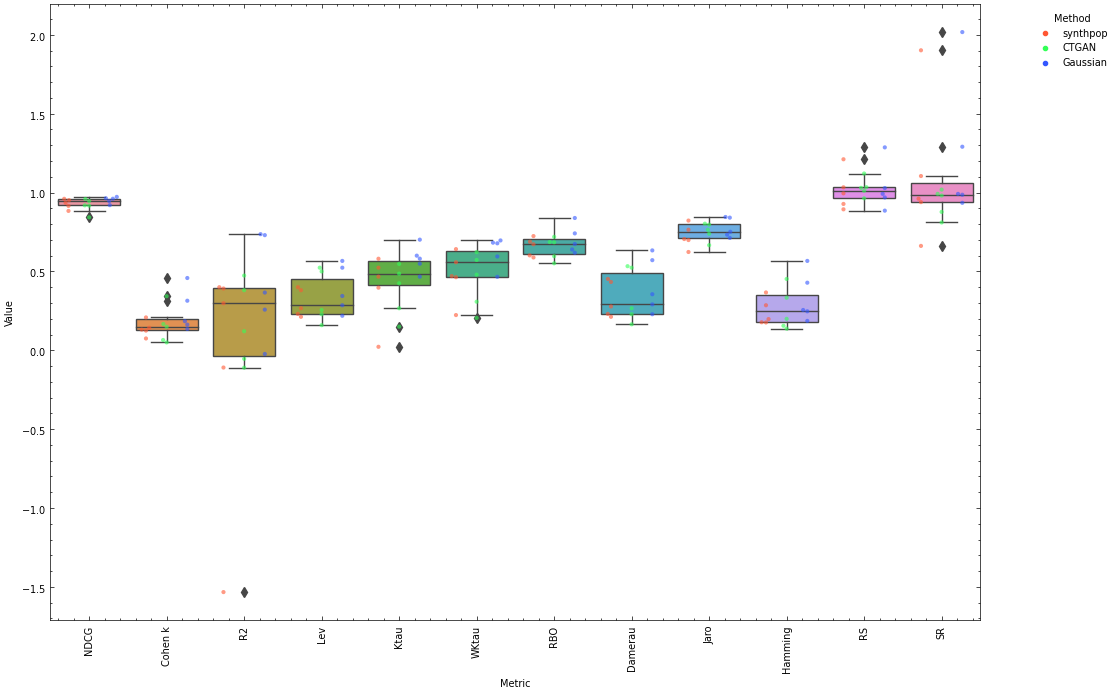
\includegraphics[scale=0.55]{figures/synthetic_violin_swarm_colored_by_group_custom.png}
\end{figure}

\Ac{cc} metrics per different models and column type was also assessed in order to help understand its advantages and disadvantages. The results can be in table~\ref{tab:method_column_type}. Finally, the imbalance of data was also assessed. We used a column with 21 different categories which was ideal to assess that impact. We mapped the percentage of each category per synthetic datasets and how they compare with the real dataset. This can be seen in figure~\ref{fig:imbalance}.
\begin{table}[h!]
    \caption{Metrics per model and variable type.}\label{tab:method_column_type}

\begin{tabular}{llcccc}
    \toprule
    Column Type & Method & Real on Real  & Real on Synth & Synth on Synth & Synth on Real \\
    \midrule
    Categorical & DT     & 0.673 (0.161) & 0.7 (0.143)   & 0.784 (0.141)  & 0.746 (0.164) \\
    Categorical & KNN    & 0.674 (0.161) & 0.7 (0.143)   & 0.783 (0.144)  & 0.747 (0.164) \\
    Categorical & LM     & 0.672 (0.161) & 0.7 (0.143)   & 0.783 (0.143)  & 0.746 (0.165) \\
    Categorical & NB     & 0.671 (0.165) & 0.7 (0.143)   & 0.783 (0.148)  & 0.747 (0.163) \\
    Categorical & RF     & 0.675 (0.158) & 0.7 (0.143)   & 0.782 (0.148)  & 0.744 (0.164) \\
    Categorical & \acs{svm}    & 0.672 (0.158) & 0.7 (0.143)   & 0.783 (0.147)  & 0.747 (0.164) \\
    \midrule
    Continuous  & DT     & 275 (719) & 324 (840) & 236 (571)  & 269 (612) \\
    Continuous  & KNN    & 316 (796) & 324 (840) & 244 (595)  & 277 (637) \\
    Continuous  & LM     & 283 (758) & 324 (840) & 242 (590)  & 272 (628) \\
    Continuous  & NB     & 288 (713) & 324 (840) & 243 (586)  & 278 (642) \\
    Continuous  & RF     & 324 (907) & 324 (840) & 242 (588)  & 276 (632) \\
    Continuous  & \acs{svm}    & 283 (727) & 324 (840) & 244 (594)  & 278 (638) \\   
    \bottomrule
    \end{tabular}

\end{table}


%TC:ignore
\begin{figure}[htbp]
    \centering
    \caption{Class distributions for an highly imbalanced category across different synthetic datasets.}\label{fig:imbalance} 
    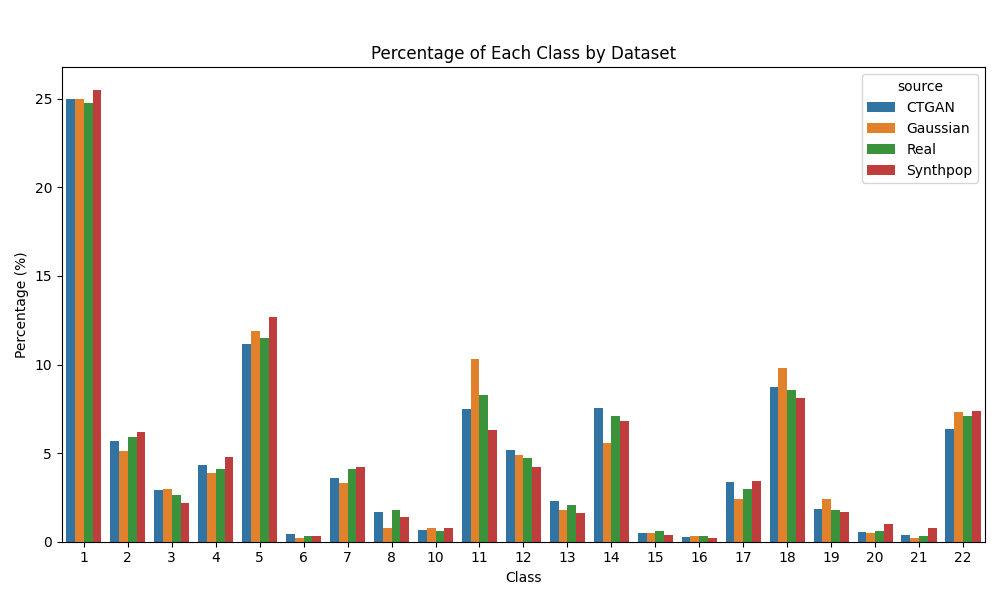
\includegraphics[scale=0.55]{figures/imbalance.png}
    \end{figure}


